\fancyhead[RO,LE]{\thepage}
\fancyfoot{} 
\chapter{Maintaining a Spatially and Temporally Coherent Active Computational Domain}
\label{chapter:temporal}

The narrow band and sparse field algorithms described in the previous chapter avoid unnecessary computation by only updating field elements near the level set surface. In this chapter I make the observation that even computations near the level set surface can be avoided in regions where the level set field has locally converged. Leveraging this insight I present an algorithm for tracking the active computational domain that is coherent in space and time.

I define the minimal set of active coordinates at time $t$ as follows:
%*******************************************************************************
\begin{equation}
    A \leftbracket t \rightbracket = \leftcbracket \boldx \in \domainphi \mid \phixt \ne \phixtmdt \rightcbracket
\label{eq:minimal}
\end{equation}
%*******************************************************************************
$A\leftbracket t \rightbracket$ is the minimal set of coordinates that must be updated at time $t$ to ensure the correctness of my algorithm because if $\phixt = \phixtmdt$, then a new value does not have to be written into the level set field at $\boldx$ and if $\phixt \neq \phixtmdt$ then I must calculate the new value $\phixt$ and write it to the level set field at $\boldx$. 

From Equation~\ref{eq:minimal} I derive two conditions, each of which is sufficient to imply that $ \boldx  \notin A \leftbracket t \rightbracket $. Both of these conditions are inexpensive to compute from local properties of the level set field and are independent of my application-specific speed function. These conditions could therefore be applied in a variety of level set simulations.

The intuition behind the first condition ${ \varsigma }_{1}$ is that computation can be avoided in regions of the level set field that are far away from the level set surface. In this sense, ${ \varsigma }_{1}$ maintains an active computational domain that is coherent in space. Formally speaking, regions that are far away from the level set surface are guaranteed to have a gradient magnitude of zero. Therefore ${ \varsigma }_{1}$ can be expressed as follows:
%*******************************************************************************
\begin{equation}
    \conditionone \equiv \leftvbracket \nabla \phixtmdt \rightvbracket = 0
\label{eq:conditionone}
\end{equation}
%*******************************************************************************
The fact that $\conditionone$ implies $\boldx \notin A\leftbracket t \rightbracket$ follows directly from  Equation~\ref{eq:levelseteq}. I note that ${ \varsigma }_{1}$ has been described previously by Lefohn et al.~\cite{Lefohn-2003-Vis,Lefohn-2004}.

The intuition behind the second condition ${ \varsigma }_{2}$ is that computation can be avoided in regions of the level set field which have locally converged, which will have a temporal derivative of zero. In this sense, ${ \varsigma }_{2}$ maintains an active computational domain that is coherent in time. I define the set $ \nx $ as the set of all coordinates in the immediate neighborhood of $ \boldx $ (including $  \boldx $ itself). I observe that if $ \phixtmdt = \phixtmtdt $, then $ \frac{ \Delta \phi \leftbracket \boldx \rightbracket }{ \Delta t } = 0 $. In other words if the level set field value is constant from one iteration to the next at $ \boldx $, then $ \phi $ is in a state of temporal equilibrium at $ \boldx $. Assuming the speed function is defined locally, the only event that could potentially disrupt this state of temporal equilibrium at $ \boldx $ is if $ \phi \leftbracket \boldn \rightbracket $ changes for some neighbor $ \boldn \in \nx $. If the level set field is in a state of temporal equilibrium in the neighborhood around $ \boldx $ at time $ t - 2 \Delta t $, then $ \boldx $ will continue to be in a state of temporal equilibrium at time $ t - \Delta t $. This leads to the following expression for ${ \varsigma }_{2}$:
%*******************************************************************************
\begin{equation}
\conditiontwo \equiv { \forall }_{ \boldn \in \nx } : \phi \leftbracket \boldn , t - \Delta t \rightbracket = \phi \leftbracket \boldn , t - 2 \Delta t \rightbracket
\label{eq:conditiontwo}
\end{equation}
%*******************************************************************************
I include a more formal derivation of ${ \varsigma }_{2}$ in Appendix~\ref{app:temporal}.
As far as I know ${ \varsigma }_2 $ is a novel contribution to the literature.

For the logical \emph{not} operator $\lnot$ I formally express the active set $A$ at time $t$ as follows:
%*******************************************************************************
\begin{equation}
A \leftbracket t \rightbracket = 
\begin{cases} 
    \domainphi                                                                                                                      & t = 0        \\
    \leftcbracket \boldx \mid \lnot \conditionone \rightcbracket                                                                    & t = \Delta t \\
    \leftcbracket \boldx \mid \lnot \conditionone \rightcbracket \cap \leftcbracket \boldx \mid \lnot \conditiontwo \rightcbracket  & t > \Delta t \\
\end{cases}
\label{eq:active}
\end{equation}
%*******************************************************************************

%*******************************************************************************
% Algorithmic Overview
\begin{figure*}[t]
\centering
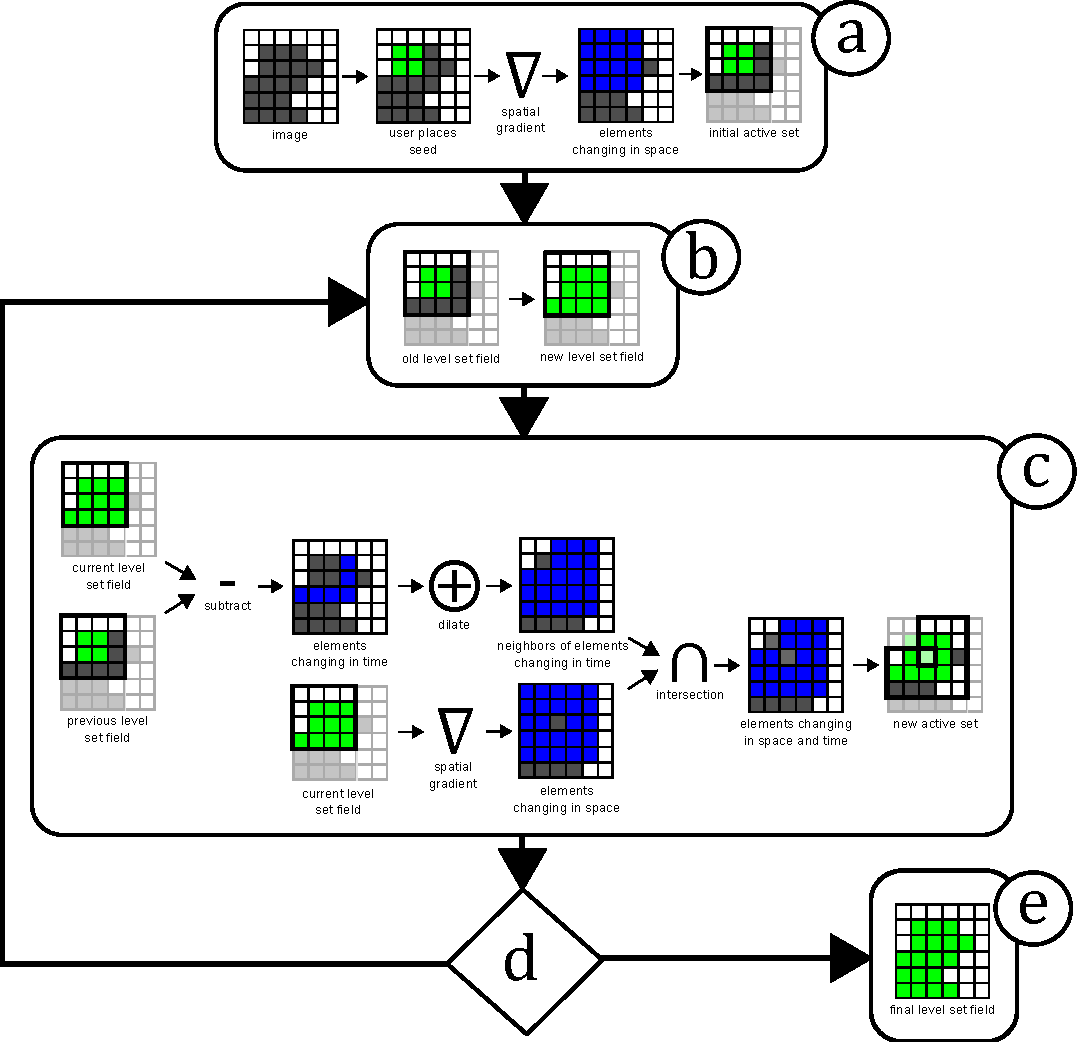
\includegraphics[width=6.0in]{figures/Algorithm.pdf}
\caption{My algorithm for tracking the active computational domain. Image data is shown in grey, currently segmented regions are shown in green, and intermediate results for computing the active computational domain are shown in blue. The active computational domain is outlined in black, and inactive elements are shown as partially transparent. The user places a seed to initialize the level set field and the initial active computational domain is determined according to the spatial derivatives of the level set field (a). During each iteration the level set field is updated at all active elements (b). The new active computational domain is computed according to the temporal and spatial derivatives of the level set field (c). If the new active computational domain is empty (d) then the segmentation has globally converged (e). Otherwise I go to (b). }
\label{fig:algorithm}
\end{figure*}
%*******************************************************************************

A diagram describing my method of tracking the active computational domain is shown in Figure~\ref{fig:algorithm} and sequential psuedo-code for this algorithm is given in Listing \ref{alg:levelset-sequential-init} and Listing \ref{alg:levelset-sequential-update}. During initialization, my algorithm initializes the level set field and then computes the initial active set according to ${\varsigma}_{1}$ only (Figure \ref{fig:algorithm}a). This is because  ${ \varsigma }_{2}$ looks for regions of the level set field that have converged with respect to time, and during initialization there are no such regions. In other words ${\varsigma}_{2}$ relies on backward time derivatives of the level set field which are initially undefined. During each iteration, my algorithm performs the level set field update on all active voxels according to Equation \ref{eq:levelseteq} (Figure \ref{fig:algorithm}b). After updating $ \phi$, the set of active voxels must itself be updated. The algorithm must then remove any voxels that are no longer active and add all voxels that have become active to the active set. Since either ${\varsigma}_1 $ or ${\varsigma}_2 $ is sufficient to exclude a voxel from the active set, both ${\varsigma}_1 $ and ${\varsigma}_2 $ must be false for the corresponding voxel to be included in the active set (Figure \ref{fig:algorithm}c). If the updated active set is empty (Figure \ref{fig:algorithm}d) then the segmentation has converged (Figure \ref{fig:algorithm}e).
During each iteration, this algorithm performs work proportional only to the size of the active computational domain. The work performed during each iteration is independent of the size of the level set field

%*******************************************************************************
\begin{Listing}[]
    \caption{Sequential pseudo code for initializing the level set field and active computational domain. The level set field is initialized to the signed and clamped distance transform relative to a user-specified seed sphere with the center \textbf{c} and the radius \textit{r}. The initial active computational domain is determined according to the spatial derivatives of the level set field on line 9.}
    \begin{algorithmic}[1]
        \FORALL { coordinates $ \boldx \in \domainphi $ } 
            \STATE { $ \phi \leftbracket \boldx , 0 \rightbracket \gets \mbox{clamp} \leftbracket \| \boldx - \mathbf{c} \|- r \rightbracket $ }
        \ENDFOR
        \STATE { $ A\leftbracket \Delta t \rightbracket \gets \emptyset $ }        
        \FORALL { coordinates $ \boldx \in \domainphi $ } 
            \STATE { $ g \gets \mbox{false} $ }
            \FORALL { coordinates $ \boldn \in \nx $ }
                \IF { $\mbox{\textbf{not }} g $ }
                    \IF { $ \phi \leftbracket \boldx , 0 \rightbracket \neq \phi \leftbracket \boldn , 0 \rightbracket $ }
                        \STATE { $ g \gets \mbox{true} $ }
                    \ENDIF
                \ENDIF
            \ENDFOR
            \IF { $ g $ }   
                \STATE { $ A \leftbracket \Delta t \rightbracket \gets A \leftbracket \Delta t \rightbracket \cup \leftcbracket \boldx \rightcbracket $ }
            \ENDIF
        \ENDFOR
    \end{algorithmic}
    \label{alg:levelset-sequential-init}
\end{Listing}
%*******************************************************************************

%*******************************************************************************
\begin{Listing}[t]
    \caption{Sequential pseudo code for updating the level set field and active computational domain until the segmentation has converged. The active computational domain is determined according to the spatial and temporal derivatives of the level set field on line 10.}
    \begin{algorithmic}[1]
        \STATE { $ t \gets \Delta t $ }
        \WHILE { $ A\leftbracket t \rightbracket \neq \emptyset $ }
            \FORALL { coordinates $\boldx \in A\leftbracket t \rightbracket $ }
                \STATE { $ \phixt \gets \phixtmdt + \Delta t F\leftbracket \boldx , t \rightbracket \leftvbracket \nabla \phixtmdt \rightvbracket $ }
            \ENDFOR
            \STATE { $ A\leftbracket t + \Delta t \rightbracket \gets \emptyset $ }            
            \FORALL { coordinates $\boldx \in A\leftbracket t \rightbracket $ }
                \STATE { $g \gets \mbox{false}$ }
                \FORALL { coordinates $\boldn \in \nx$ }
                    \IF { $ \phixt \neq \phi \leftbracket \boldn , t \rightbracket \mbox{\textbf{ and }} \phixt \neq \phixtmdt $ }
                        \STATE { $ g \gets \mbox{true} $ }
                        \STATE { $ A\leftbracket t + \Delta t \rightbracket \gets A\leftbracket t + \Delta t \rightbracket \cup \leftcbracket \boldn \rightcbracket $ }      
                    \ENDIF
                \ENDFOR
                \IF { $ g $ }   
                    \STATE { $ A\leftbracket t + \Delta t \rightbracket \gets A\leftbracket t + \Delta t \rightbracket \cup \leftcbracket \boldx \rightcbracket $ }      
                \ENDIF
            \ENDFOR
            \STATE { $ t \gets t + \Delta t $ }
        \ENDWHILE
    \end{algorithmic}
    \label{alg:levelset-sequential-update}    
\end{Listing}
%*******************************************************************************

